% ============================================== %
%
% Methodology.tex
%
%% ============================================== %
\chapter{Methodology} \label{chap:methodology}
\hypersetup{colorlinks=true, linkcolor=red}

    In this chapter, the methodology used to split the data and train the models is presented. In addition, the fundamental concepts behind the models used are explained.

    \section{Overview of the models}

        In this comparative study a total of ten popular models are selected for analysis of their perfomance on Kinect-based data.

        \subsection{Scikit-learn library}  

            Scikit-Learn is a Python library designed for Machine Learning, it offers a wide range of \textit{state of the art} algorithms for medium scale supervised and unsupervised problems. It emphasizes ease of use, perfomance, and API consistency, targeting non specialists with its high level approach. It stands out for its minimal dependecies and broad accessibility, being distributed under the simplified BSD license. It integrates well with the Python ecosystem, making it highly desirable for both academic and commercial applications \cite{scikit-learn}.

        \subsection{Models selection}

        The models presented in Table \ref{tab:movements_table} are used for the classification task. Selected on a basis of popularity and performance, these models are widely used in the machine learning community. The models are implemented using the \textit{scikit-learn} library and it's functions for training, testing and evaluating\cite{sklearn_api}. 

        \newpage 

        \begin{table}[htbp]
            \centering
            \begin{tabular}{@{}clcl@{}}
                \toprule
                \multicolumn{4}{c}{\textbf{Model Name}} \\
                \midrule
                1 & Support Vector Machine & 6 & Linear Discriminant Analysis \\
                2 & Gaussian Naive Bayes & 7 & Multi-Layer Perceptron \\
                3 & Random Forest & 8 & K-Nearest Neighbors \\
                4 & Gradient Boosting & 9 & AdaBoost \\
                5 & Logistic Regression & 10 & Decision Tree \\
                \bottomrule
            \end{tabular}
            \caption{Models selected for use in this thesis.}
            \label{tab:movements_table}
        \end{table}
    
    \section{Models analysis}
        
        In this section the models that performed best in the Chapter \ref{chap:results_and_discussion} are analyzed. The models are analyzed in terms of their implementation.

        \subsection{Random forest}
           Also known as \textit{random decision forests}, is a method of ensemble learning used for classification, regression, and various other tasks. It involves building numerous decision tress during the training phase. In classification tasks, the class chosen by the majority of trees is the output of the random forest \cite{ho_random_1998}.

           \begin{figure}[H]
            \centering
            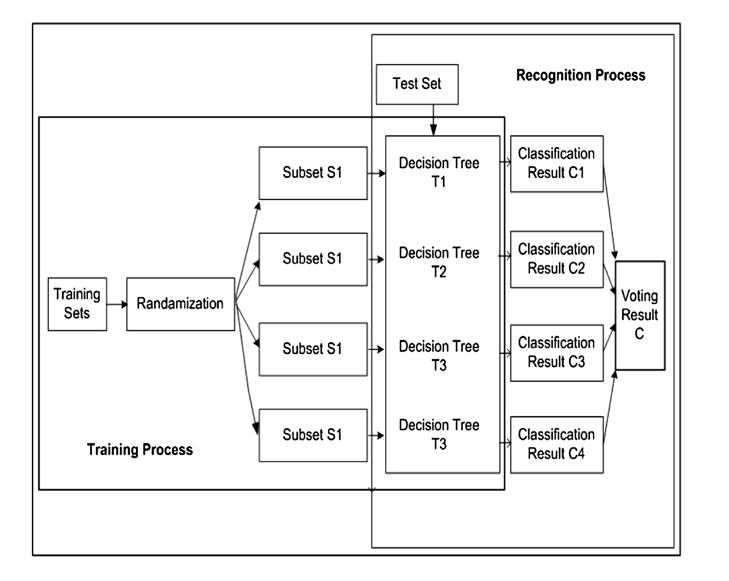
\includegraphics[width=.7\textwidth]{../src/resources/rf_image.png}
            \caption{
                The process starts with multiple training sets that undergo randomization to create several subsets S1. Each subset is used to train a separate decision tree (T1 to T3). The trained trees are then used to make predictions on a test set. The predictions (C1 to C4) from each tree are aggregated through a voting mechanism to produce a final classification result (C). This ensemble approach leverages multiple models to improve prediction accuracy and robustness. \cite{parmar_review_2019}.
            }
            \label{fig:random_forest}
            \end{figure}

            The main steps involved in building a random forest classifier are as follows:
           
            \begin{enumerate}
                \item Define $M$ as the number of features in each subset.
                \item Randomly select a feature subset $\theta_k$ from the full set, distinct from proceding subset $\theta_{1},..., \theta_{k-1}$.
                \item Train decision trees on each $\theta_k$ denoted as $h(X, \theta_k)$.
                \item Iteratively select new $\theta_k$ subsets and train untill all tress are built.
                \item Classify test data by majority vote of all trees in the forest.
            \end{enumerate}

            Random forests consist of numerous decision trees. Randomization in tree building—through sampling instances and feature subsets via bagging—enhances diversity, reducing overfitting and improving generalization. Feature subsets $\theta_k$​ are chosen by bagging, and the importance of features is ranked by their impact on the model's accuracy. The "strength" and "correlation" of the forest are influenced by $M$, with optimal values providing a balance. The random forest's efficiency is due to its parallel structure, accelerating classification significantly \cite{parmar_review_2019}.
            
        \subsection{Gradient boosting}
            Gradient boosting is a machine learning method that refines predictions iteratively, combining the strengths of simple models, like decision trees, into a more accurate ensemble. Each iteration, represented by $F_m(x)$, improves upon the last by adding a weighted decision tree $\rho_m h_m(x)$ that addresses the previous errors. The process follows the \textit{principle of gradient descent}, where $h_m(x)$ is trained to predict the negative gradient of the loss function, effectively reducin the residual between the predicted and true values. The ensemble begins with a single model $F_0(x)$, which is updated by the formula:
            \begin{equation}
                F_m(x) = F_{m-1}(x) + \rho_m h_m(x)
            \end{equation}
            The aim is to minimize the loss function $L(y, F_m(x))$ at each step, ensuring the model's prediction become progressively more accurate \cite{bentejac_comparative_2021}.
            \begin{figure}[H]
                \centering
                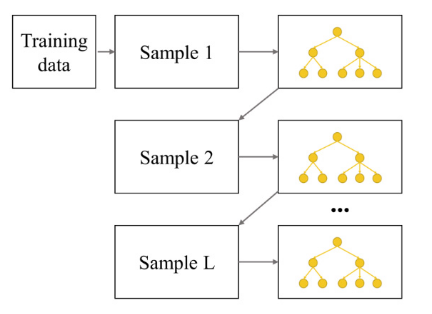
\includegraphics[width=.5\textwidth]{../src/resources/boosting.png}
                \caption{
                    Starting with the training data, the algorithm iteratively trains decision trees (Sample 1 to Sample L). Each tree is trained on the errors of the previous ones, aiming to correct these mistakes. Over multiple iterations, each tree improves the model's predictions, and the final output is the combined effort of all the trees, effectively reducing prediction errors. \cite{cha_comparison_2021}.
                }
                \label{fig:gradient_boosting}
            \end{figure}

        \newpage

        \subsection{Logistic regression}
            Logistic regression is a statisstical model used for binary classification that predicts the probability of a binary response based on one or more predict variables. It applies a logistic function to a linear combination of the input features to produce a value between 0 and 1, interpreted as the probability of the instance being in the positive class.
            Equation \ref{eq:logistic_regression} shows the logistic function for binary classification.

            \begin{equation} \label{eq:logistic_regression}
                P(Z) = \frac{1}{1 + e^{-(\beta_0 + \beta_1 x)}}
            \end{equation}

            In multi class classification, the one-vs-rest approach involves training a separate logistic regression classifier for each classh to distinguish that class from all other classes. For each classifier, the class it's designed to identify is treated as the positive class, and all others are lumped into a single negative class.
            The logistic function is the same as for binary classification, presented in Equation \ref{eq:logistic_regression}. It is applied multiple times, one for each class.
            
            \begin{figure}[htbp]
                \centering
                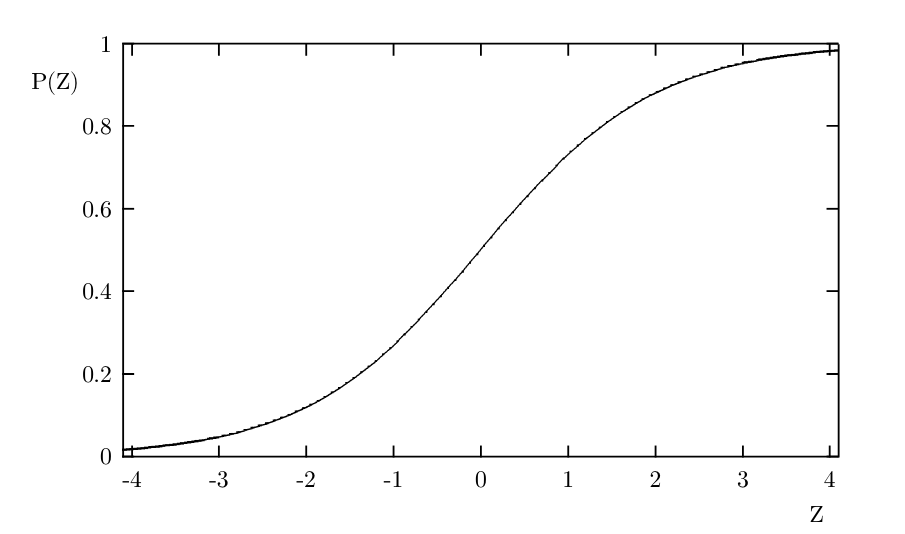
\includegraphics[width=.8\textwidth]{../src/resources/logistic.png}
                \caption{
                    The horizontal axis labeled 'Z' represents the input variable (which is a linear combination of the features), and the vertical axis labeled 'P(Z)' represents the probability that the outcome is the positive class. The curve transitions smoothly from 0 to 1, with an inflection point at Z=0, where P(Z) = 0.5. This S-shaped curve allows logistic regression to convert continuous predictions into a probability between 0 and 1, facilitating binary classification \cite{cramer_origins_2002}.
                }
                \label{fig:logistic_regression}
            \end{figure}

        \subsection{Linear discriminant analysis}
            Linear Discriminant Analysis (LDA) is a method used in statistics and machine learning to find a linear combination of features that separates two or more classes of objects or events. It does so by maximizing the ratio of between-class variance to the within-class variance in any particular data set, thereby ensuring maximum separability.

            In the binary class, the goal is to find a linear combination $w$ tjat separates the classes. This involves computing the mean vectors $m_1$ and $m_2$ for each class, the within class scatter matrix $S_W$, and the between class scatter amtix $S_B$. The linear discriminants are then the eigenvectors of $S_W^{-1}S_B$ \cite{xanthopoulos_linear_2013}. 

            \begin{figure}[H]
                \centering
                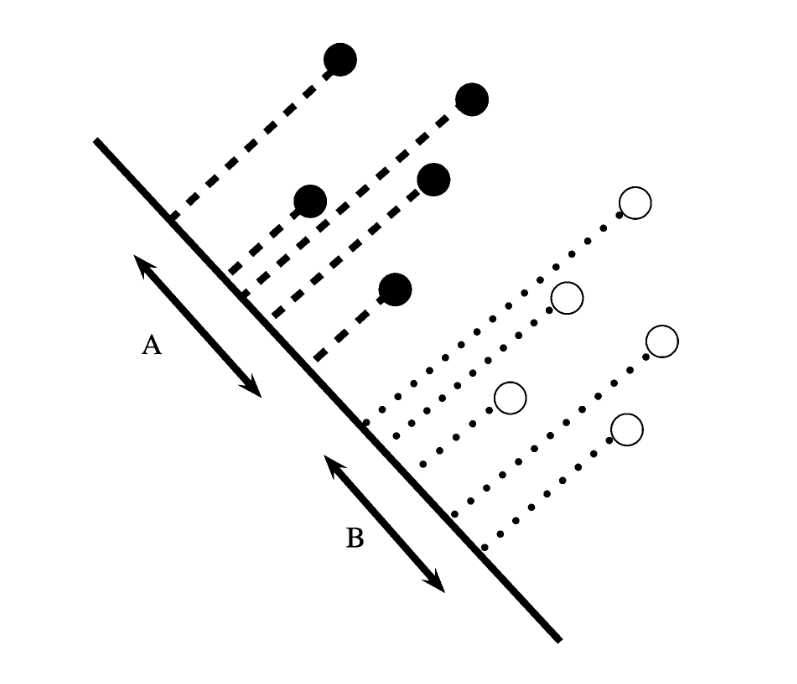
\includegraphics[width=.6\textwidth]{../src/resources/lda.png}
                \caption{
                    Intuition behind LDA. Data samples in two dimensions ae projected in a lower dimension space. The line has to be chosen so that the projection maximizes the "separability" of the projected samples. \cite{xanthopoulos_linear_2013}.
                }
                \label{fig:linear_discriminant_analysis}
            \end{figure}

            For multi class problems, the same principle applies but extends to multiple classes. The within class scatter matrix $S_W$ and between class scatter matrix $S_B$ are computed considering all classes, and the objective is to find the linear discriminants that maximize the separation among all classes.  

            The simplicity and effectiveness of LDA, especially under the assumptions of normality and equal class covariances, make it a powerful tool for classification \cite{balakrishnama_linear_nodate}.

        \subsection{Multi layer perceptron}
            Multi-layer perceptron architecture include at least three layers, an input layer, an output layer, and one or more hidden layers, each composed of nodes with nonlinear activation functions \cite{svozil_introduction_1997}. They are referred to as "vanilla" neural networks \cite{hastie_elements_2009}.

        \begin{equation}\label{eq:tan}
            y(v_i) = \text{tanh}(v_i) 
        \end{equation}

        \begin{equation}\label{eq:sigmoid}
            y(v_i) = (1+e^{-v_i})^{-1} 
        \end{equation}

            A linear function can simplify multiple layers to a two layer model, mapping weighted inputs to a neuron outputs. Nonlinear activation functions, like the hyperbolic tangent \ref{eq:tan} ranging from -1 to 1, or the sigmoid function \ref{eq:sigmoid} ranging from 0 to 1, are used to introduce nonlinearity into the model. This allows the model to learn complex patterns in the data.

        \newpage

        In the context of MLP, complete connectivity is maintained, every node within a given layer connects to every node in the subsequent layer via weighted connections. \\
        The learning process involves the dynamic adjustment of connection weights following the processing of each data point. This adjustment is made in response to the disparity between the actual output and the expected outcome, with the goal of minimizing the error.

        \begin{figure}[H]
            \centering
            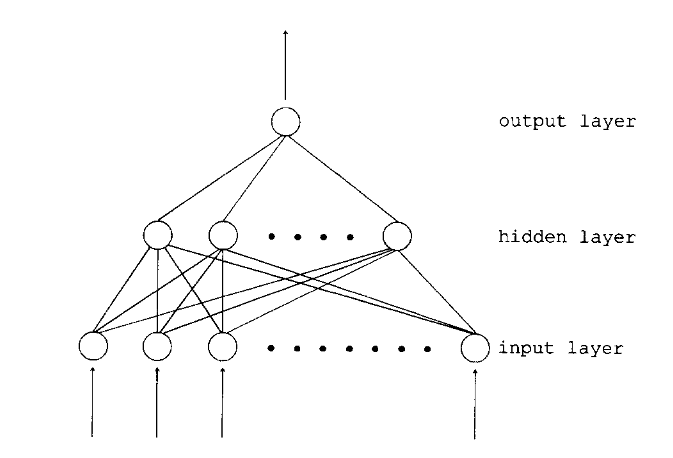
\includegraphics[width=.7\textwidth]{../src/resources/feedforward.png}
            \caption{
                Feed forward network consisting of an input layer, one or more hidden layers, and an output layer. \cite{svozil_introduction_1997}
            }
            \label{fig:multi_layer_perceptron}
        \end{figure}
    
    \newpage
        
        
    \section{Data splitting methods}
        
            Due to the structure of the data, the traditional approach of splitting the data into training and testing sets is not effective. Two different approaches will be presented, one ineffective and one effective.

            \subsection{Traditional} \label{sec:badsplit}
                        
                    The data is split into 70\% training and 30\% testing following the traditional approach used in Machine Learning literature. The code snippet in \ref{lst:badsplit} demonstrates this approach. 
            
\begin{lstlisting}[
    caption={Traditional approach to splitting the data into training and testing sets.}, 
    label={lst:badsplit},
    ]            
    def split_data(data: pd.DataFrame) -> tuple:        
        X = data.iloc[:, :-1].values
        y = data.iloc[:, -1].values
        
        X_train, X_test, y_train, y_test = train_test_split(
            X, y, test_size=0.33, random_state=42)
        
        return X_train, X_test, y_train, y_test
\end{lstlisting}
                
                    Figure \ref{fig:badsplit} visualization demonstrates why this approach is ineffective. Every row in the dataset is associated with a specific patient. The data is split randomly, so there is a chance that the same patient will appear in both the training and testing sets. This means that the model will be trained on data that it will also be tested on, which will result in a high accuracy score. However, this is not a good indicator of the model's performance on unseen data.

                    \begin{figure}[H]
                        \centering
                        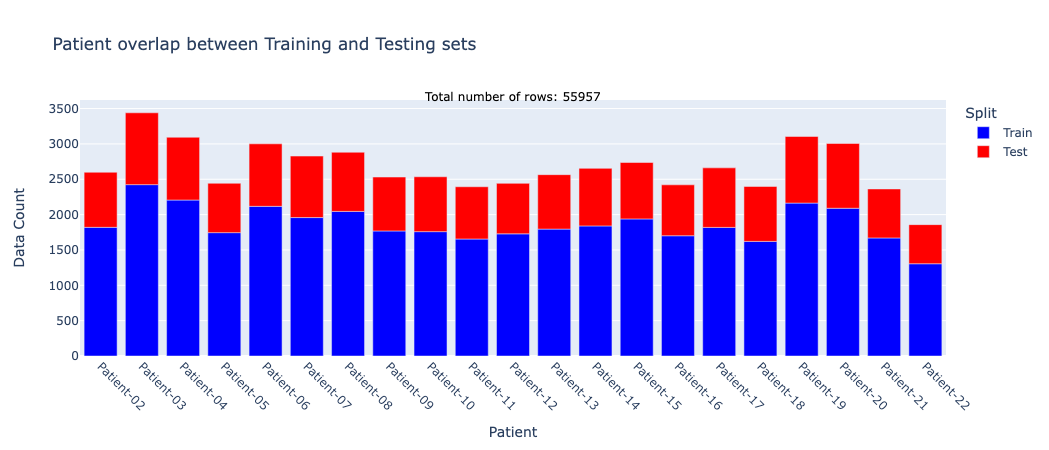
\includegraphics[width=1.0\textwidth]{../src/resources/bad_split.png}
                        \caption{
                            Visualization of the ineffective data splitting approach.
                        }
                        \label{fig:badsplit}
                    \end{figure}
        
                    \newpage

            \subsection{Effective} \label{sec:goodsplit}
            Data is split into training and testing sets based on the patient's unique ids. The patients are split into training and testing sets, and then the data is split based on the patient's unique ids.  The code snippet in \ref{lst:goodsplit} demonstrates this approach.

\begin{lstlisting}[
    caption={Effective approach to splitting the data into training and testing sets.}, 
    label={lst:goodsplit}]
    def split_data(data: pd.DataFrame) -> tuple:    
        unique_patients = data['patient'].unique()

        train_patients, test_patients = train_test_split(unique_patients, test_size=0.3, random_state=42)

        train_data = data[data['patient'].isin(train_patients)]
        test_data = data[data['patient'].isin(test_patients)] 

        X_train = train_data.drop(columns=['label', 'patient'])
        y_train = train_data['label']

        X_test = test_data.drop(columns=['label', 'patient'])
        y_test = test_data['label']
        
        return X_train, X_test, y_train, y_test
\end{lstlisting}

            Figure \ref{fig:goodsplit} visualization demonstrates why this approach is effective. The data is split based on the patient's unique ids, so the model will be trained on data that it will not be tested on. This means that the model will be tested on unseen data, which is a good indicator of the model's performance.

            \begin{figure}[H]
                \centering
                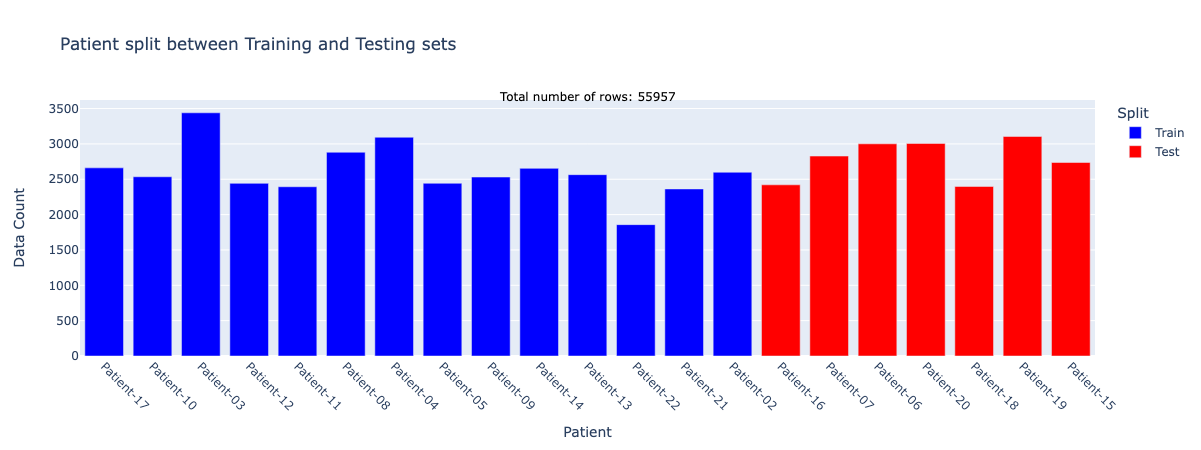
\includegraphics[width=1.0\textwidth]{../src/resources/good_split.png}
                \caption{
                    Visualization of the effective data splitting approach.
                }
                \label{fig:goodsplit}
            \end{figure}

    \newpage
            
            \subsection{Sequential} \label{sec:seqsplit}
            Data is split into training and testing sets based on the patient's unique ids, then the sets are split into sequences. Where each sequence represents the stack of frames that make up a movement. The code snippet in \ref{lst:seqsplit} demonstrates the splitting into sequences of the data. 

\begin{lstlisting}[
    caption={Effective approach to splitting the data into training and testing sets.}, 
    label={lst:seqsplit}]                
    def sequences(df: pd.DataFrame, feature_columns: list, sequence_column: str) -> tuple:
        sequences = []
        labels = []
        current_sequence = []
        current_check = None

        for _, row in df.iterrows():
            check = row[sequence_column]
            label = row['label']
            if check != current_check and current_sequence:
                sequences.append(np.array(current_sequence))
                labels.append(label)
                current_sequence = []
            current_sequence.append(row[feature_columns].to_numpy())
            current_check = check

        if current_sequence: 
            sequences.append(np.array(current_sequence))
            labels.append(label)

        return sequences, labels
\end{lstlisting}

            Figure \ref{fig:seqsplit} visualization shows how for each movement the data is split into sequences for training and testing. However, using only this approach is not enough, as the sequences are of different lengths due to each movement having a variable number of frames. This means that the sequences cannot be used as input for the models since they require a fixed input size. 
        
            \begin{figure}[H]
            \centering
            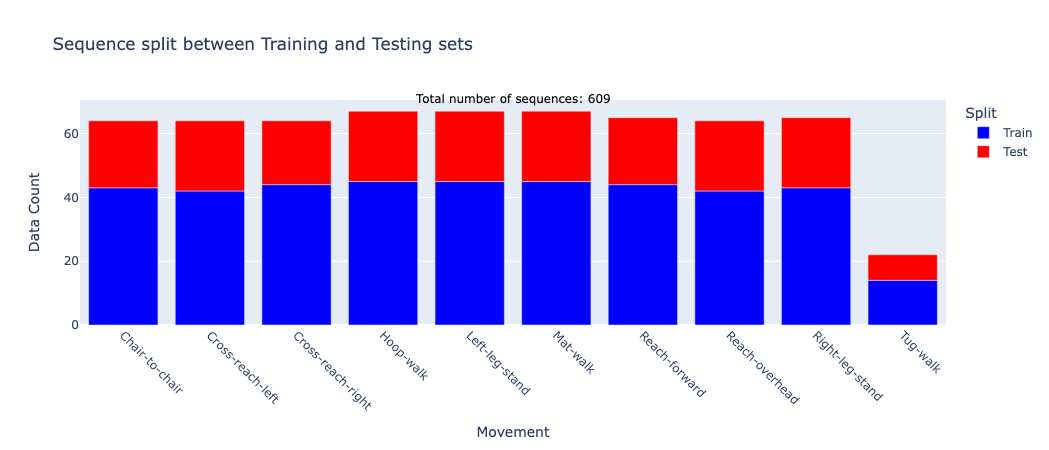
\includegraphics[width=1.0\textwidth]{../src/resources/seq_split.png}
            \caption{
                Visualization of the sequences splitting approach.
            }
            \label{fig:seqsplit}
        \end{figure}

        \newpage 

        To solve the variable length problem, the sequences are aggregate into a single featurere vector. The code snippet \ref{lst:seqagg} demonstrates this approach. In Figure \ref{fig:seqlength}, the length of the sequences before and after aggregation is visualized. The aggregation is done by calculating the mean of each feature for each frame in the sequence. This results in a single feature vector for each sequence, which can be used as input for the models.

\begin{lstlisting}[
    caption={Sequences are aggregated into a single feature vector.}, 
    label={lst:seqagg}]                
    def aggregate_features(sequences: list) -> np.ndarray:
            return np.array([np.mean(sequence, axis=0) if sequence.size != 0 else np.zeros(sequence.shape[1]) for sequence in sequences])
\end{lstlisting}
        
However, there are some drawbacks to this approach. The aggregation results in a loss of information, as the data is no longer represented as a sequence of frames. In addition, the aggregation results in a loss of the temporal information, as the order of the frames is lost. This means that the models will not be able to learn the temporal patterns in the data.

\begin{figure}[H]
    \centering
    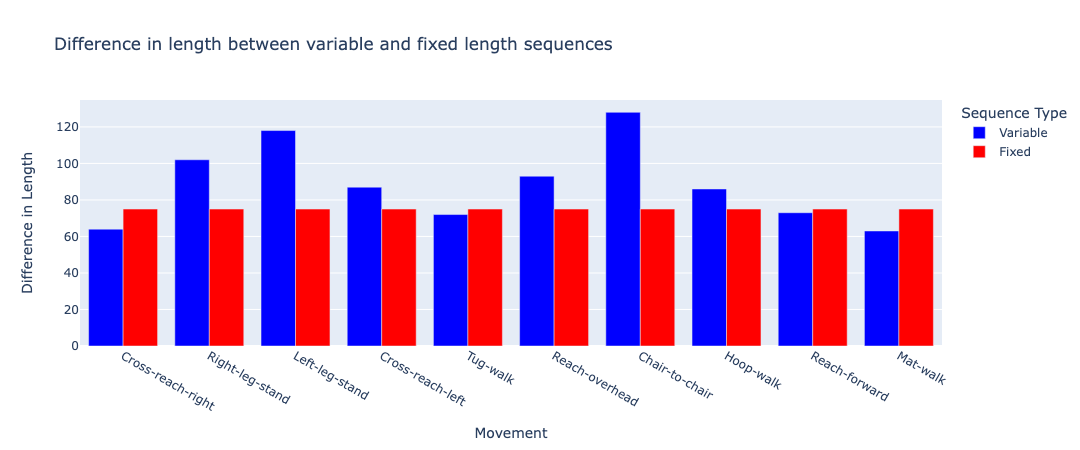
\includegraphics[width=1.0\textwidth]{../src/resources/plots/length.png}
    \caption{
        Visualization of the length of the sequences before and after aggregation.
    }
    \label{fig:seqlength}
\end{figure}

    \newpage
    
    \section{Feature engineering} \label{sec:feature_engineering}
        
        Feature engineering is the final approach used in this thesis. It is used to extract new features from the raw Kinect skeleton data, in order to improve the performance of the models.

        \subsection{Overview}

            This process is implemented  in order to improve the performance of the models due to them not being able to differentiate well between the movements based on the raw data. This allows to obtain data that is more informative and easier to interpret. The features extracted from the Kinect Skeleton data are presented in Table \ref{tab:features_table}.

        \begin{table}[htbp]
            \centering
            \begin{tabular}{@{}clcl@{}}
                \toprule
                \multicolumn{4}{c}{\textbf{Features}} \\
                \midrule
                1 & Duration & 2 & Area \\
                3 & Velocity & 4 & Distance \\
                5 & Vertical Displacement & 6 & Horizontal Displacement \\
                7 & Forward Displacement &  & \\
                \bottomrule
            \end{tabular}
            \caption{Features extracted from the Kinect Skeleton data.}
            \label{tab:features_table}
        \end{table}

        \subsection{Calculation Methods}

            The features presented in Table \ref{tab:movement_table} are calculated using the following methods. For each of the features, the method used to calculate it is presented, along with a brief description.

            \begin{table}[ht]
                \centering
                \begin{tabular}{@{}clcl@{}}
                    \toprule
                    \multicolumn{4}{c}{\textbf{Body parts selected}} \\
                    \midrule
                     Head & ShoulderLeft & ShoulderRight & SpineShoulder \\
                     SpineMid & SpineBase & ElbowLeft & ElbowRight \\
                     WristLeft & WristRight & HipLeft & HipRight \\
                     KneeLeft & KneeRight & AnkleLeft & AnkleRight \\
                    \bottomrule
                \end{tabular}
                \caption{Selected body parts from the Kinect Skeleton data joints.}
                \label{tab:body_parts_table}
            \end{table} 

            \subsubsection{Duration}

                The duration is defined as how long it takes for the movement to be performed from start to finish. It is calculated as the difference between the maximum and minimum datetime column values. The difference is calculated in seconds.

                \begin{equation}\label{eq:duration}
                    \text{Duration} = (\text{{max\_datetime}} - \text{{min\_datetime}})
                \end{equation}
            
            \subsubsection{Area}

                The area is defined as the aggregate area of convex hulls formed by the trajectories of selected body parts. It operates by extracting the (x,y,z) coordinates for each specified body part, constructing a convex hull for these points, and then calculating the hull's volume.

                \begin{equation}\label{eq:area}
                    \text{Area} = \sum_{i=0}^{n} \text{Volume}(\text{Hull}(P_i))
                \end{equation}
            
                In Equation \ref{eq:area}, $P_i$ is the set of points representing the trajectory of body part $i$ in 3D space, where $i \in \{1, 2, ..., n\}$ for $n$ body parts. The convex hull of $P_i$ is denoted as $\text{Hull}(P_i)$, is the smallest convex set that contains all points in $P_i$. The volume (area in 3D) of $\text{Hull}(P_i)$ is calculated using the formula for the volume of a convex polyhedron, which depends on the vertices of the hull. The total area calculated is the sum of the volumes of these convex hulls for app specified body parts.
                
        \begin{lstlisting}[caption={Area calculation method using the ConvexHull class from the SciPy library.}] 
        def area(df: pd.DataFrame, body_parts: list) -> float:
            def calculate(points: np.ndarray) -> float:
                hull = ConvexHull(points)
                return hull.volume
            trajectories = {}
            for column in body_parts:
                body_part = column.split('.')[0]
                trajectory = df[[body_part + '.px', body_part + '.py', body_part + '.pz']].values
                trajectories[body_part] = trajectory
            temp = {}
            for body_part, trajectory in trajectories.items():
                temp[body_part] = calculate(trajectory)
            return sum(temp.values())
        \end{lstlisting}

                \begin{figure}[H]
                    \centering
                    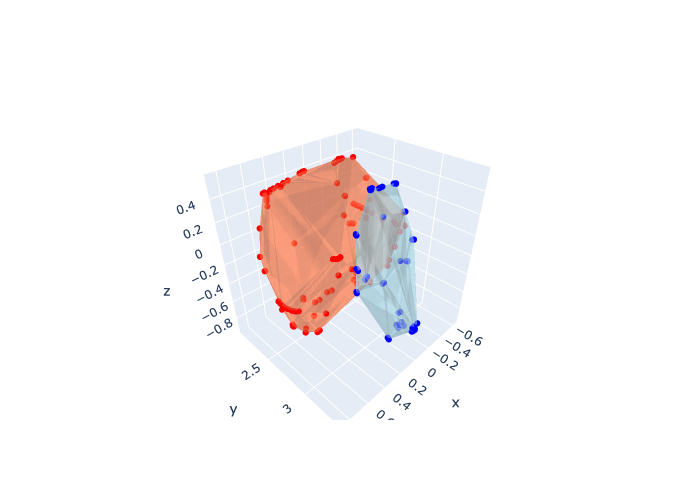
\includegraphics[width=.6\textwidth]{../src/resources/area.png}
                    \caption{
                        Visualization of the area occupied by two movements, the red area represents \textit{Chair to Chair} while the blue area represents \textit{Right Leg Stand}. 
                    }
                    \label{fig:area}
                \end{figure}
            
            \subsubsection{Velocity}
                
                The velocity is defined as the rate of change of the displacement over time. It is calculated as the square root of the sum of the squared displacement over time difference for each axis. 

                \begin{equation}\label{eq:velocity}
                    \text{velocity} = \sqrt{\left(\frac{\text{displacement}_x}{\text{time difference}}\right)^2 + \left(\frac{\text{displacement}_y}{\text{time difference}}\right)^2 + \left(\frac{\text{displacement}_z}{\text{time difference}}\right)^2}
                \end{equation}

                               
        \begin{lstlisting}[
            caption={Velocity calculation method.}, 
            label={lst:vertical_displacement}],     
    def velocity(df: pd.DataFrame) -> float:
        first = df.iloc[0]
        last = df.iloc[20]
        start = first['datetime'].split('_')[1].split('.')[0]
        end = last['datetime'].split('_')[1].split('.')[0]
        diff = pd.to_datetime(end) - pd.to_datetime(start)
        velx = last['Head.px'] - first['Head.px'] / diff.total_seconds()
        vely = last['Head.py'] - first['Head.py'] / diff.total_seconds()
        velz = last['Head.pz'] - first['Head.pz'] / diff.total_seconds()
        return math.sqrt(velx**2 + vely**2 + velz**2)
        \end{lstlisting}

                \begin{figure}[H]
                    \centering
                    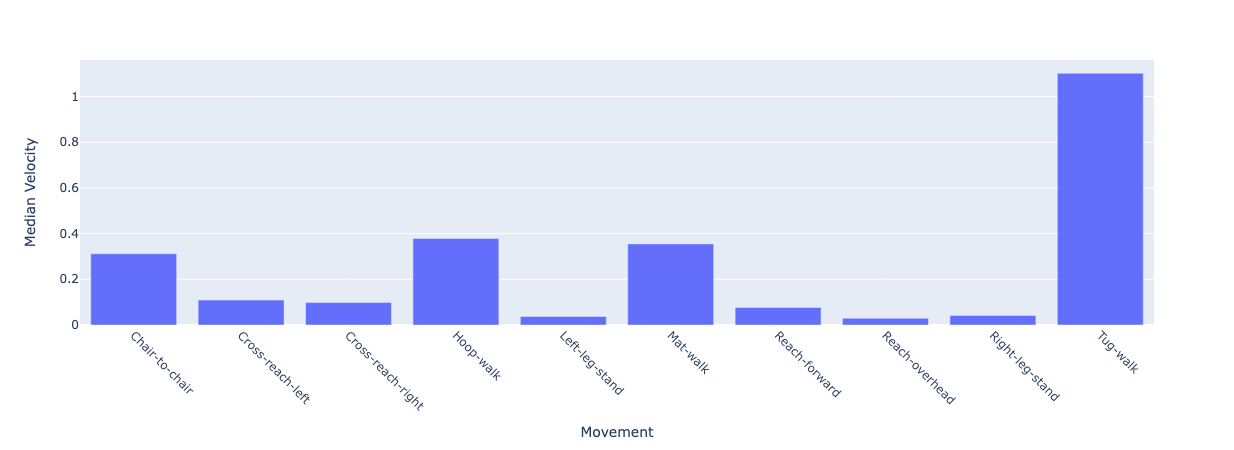
\includegraphics[width=1.0\textwidth]{../src/resources/velocity.png}
                    \caption{
                       Visualization of the median velocity of each movement in the dataset. This shows how the velocity varies between the movements and can be used to differentiate between them.
                    }
                    \label{fig:velocity}
                \end{figure}

            \subsubsection{Distance}

                The distance is defined the total 3D Euclidean distance between consecutive points representing the position of a body part, typically the head. It is calculated by taking each pair of consecutive rows in the dataset, computing the distance between their (x,y,z) head positions in 3D space using the Euclidean distance formula, and summing  up these distances to find the overall total distance covered by the body part in the sequence.

                \begin{equation}
                    \text{Distance} = \sum_{i=0}^{n-1} \sqrt{(x_{i+1} - x_i)^2 + (y_{i+1} - y_i)^2 + (z_{i+1} - z_i)^2}
                \end{equation}

                \begin{lstlisting}[
                    caption={Distance calculation method.}, 
                    label={lst:vertical_displacement}],     
    def calculate(row1: pd.Series, row2: pd.Series, point="Head") -> float:
        return np.sqrt((row2[f'{point}.px'] - row1[f'{point}.px'])**2 +
                        (row2[f'{point}.py'] - row1[f'{point}.py'])**2 +
                        (row2[f'{point}.pz'] - row1[f'{point}.pz'])**2)
    
    def distance(df: pd.DataFrame) -> float:
        return sum(calculate(df.iloc[i], df.iloc[i+1]) for i in range(len(df) - 1))
                \end{lstlisting}
            \subsubsection{Time steps displacement}
                The following joints: \textit{AnkeLeft}, \textit{AnkleRight}, \textit{WristLeft}, \textit{WristRight}, \textit{SpineMid} have been selected for the calculation of the displacement. These joints have been selected as they are the most informative for the movements in the dataset. \\

                Time steps displacement is defined as the total change in the position of a body part from the start to the end of the movement. It is calculated by taking the absolute differences in the positions of the body part between consecutive time steps, and then summing up these differences over all time steps.

                \begin{equation} \label{eq:displacement}
                    \text{Time steps displacement} = \sum_{t=1}^{n} \left| P(t) - P(t-1) \right|)
                \end{equation}
                In Equation \ref{eq:displacement}, $P$ is a placeholder for the axis positions of the body part, and $t$ is the time step. 
                \begin{enumerate}
                    \item \textbf{Vertical} is calculated by taking the $Y$ axis positions.
                    \item \textbf{Horizontal} is calculated by taking the $X$ axis positions.
                    \item \textbf{Forward} is calculated by taking the $Z$ axis positions.
                \end{enumerate}
               
        \begin{lstlisting}[
    caption={Vertical time steps displacement calculation method.}, 
    label={lst:vertical_displacement}],     
    def vertical(df: pd.DataFrame, joint: str) -> float:
        df['vertical_diff'] = df[f'{joint}.py'].diff().abs()
        total_vertical = df['vertical_diff'].sum()
        return total_vertical
        \end{lstlisting}
\cleardoublepage